\documentclass[letter,11pt]{article}

\usepackage[spanish,es-nodecimaldot]{babel}
\usepackage[utf8]{inputenc}

\usepackage{lmodern}
\usepackage[T1]{fontenc}
\usepackage{textcomp}

\usepackage{framed}
\usepackage[svgnames]{xcolor}
\colorlet{shadecolor}{Gainsboro!50}

\usepackage{enumitem}
\usepackage{graphicx}
\usepackage{pstricks}

\usepackage{anysize}
\marginsize{3cm}{2cm}{2cm}{3cm}

\usepackage{siunitx}
\usepackage{amsmath}
\usepackage{array}
\usepackage{alltt}

\usepackage{fancyhdr}
\usepackage{lastpage}
\pagestyle{fancy}
\fancyhf{}
\fancyhead[LE,RO]{Mecánica de fluidos}
\fancyfoot[CO,CE]{\thepage\ de \pageref{LastPage}}

\special{papersize=215.9mm,279.4mm}

\usepackage[
    pdfauthor={Carlos Eduardo Caballero Burgoa},%
    pdftitle={Mecánica de fluidos},%
    pdfsubject={Practica 02},%
    colorlinks,%
    citecolor=black,%
    filecolor=black,%
    linkcolor=black,%
    urlcolor=black,
    breaklinks]{hyperref}
\usepackage{breakurl}

\newcommand{\blankpage}{
\newpage
\thispagestyle{empty}
\mbox{}
\newpage
}

\renewcommand{\arraystretch}{1.2}

\begin{document}

\begin{center}
    {\large \bf{\underline{Practica \#02}}}
\end{center}
\vspace{0.25cm}

\begin{enumerate}
\item \textbf{En la figura se muestra los elementos básicos de una prensa
hidráulica. El área transversal del piston $1$ al cual se le aplica una fuerza
$F1$ es $650mm^2$. El piston $1$ es accionado por un mecanismo de palanca el
cual tiene una relación de fuerzas de $8:1$. El piston $2$ en el cual actua la
fuerza $F2$ tiene un area transversal de $96774m^2$. Calcular la fuerza $F2$ si
se aplica una fuerza de $90N$ en el mecanismo de palanca.}

\begin{figure}[!h]
\centering
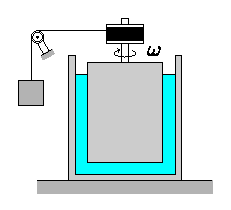
\includegraphics[scale=1.35]{figura01.eps}
\end{figure}

\item \textbf{Hallar la presión en el tanque $A$ y cual es la presion del aire
en el tubo para la siguiente figura. Calcular la presión en el tanque $A$ y la
presión del aire en el tubo si se cambia el agua por mercurio.}

\begin{figure}[!h]
\centering
\includegraphics[scale=1.50]{figura02.eps}
\end{figure}

\item \textbf{Se tienen dos tanques separados como se muestra en la figura, el
tanque $A$ contiene aire presurizado y en el compartimiento $B$ hay un liquido
de densidad relativa de $0.6$. Determinar la altura $h$ en el manometro sabiendo
que la presion atmosferica es $101.3kPa$, tener en cuenta que el manometro
instalado en el compartimiento $A$ indica una presion de $3.5kPa$.}

\begin{figure}[!h]
\centering
\includegraphics[scale=2.00]{figura03.eps}
\end{figure}

\item \textbf{La figura muestra una carcasa semiesferica llena de aire que esta
en el fondo del oceano a una profundidad de $10m$. Un barometro localizado
dentro a la carcasa presenta una columna de mercurio con una altura maxima de
$765mm$ y el tubo en $U$ muestra una lectura de $735mm$ de mercurio, utilizando
estos datos determinar cual es el valor de la presion atmosferica, en otras
palabras la presion en la superficie libre del oceano.}

\begin{figure}[!h]
\centering
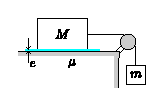
\includegraphics[scale=2.00]{figura04.eps}
\end{figure}

\item \textbf{Cuando se requiere una gran precision en la medicion de presiones
se utiliza un micromanometro. En el sistema se utilizan dos liquidos no
miscibles con pesos especificos $\gamma_1$ y $\gamma_2$ respectivamente. Se
supone que los fluidos en los tanques $E$ y $B$, cuya diferencia de presión
quiere medirse, son gasos con pesos especificos insignificantes. Calcule la
diferencia de presión $P_E$ y $P_B$ en funcion de $\delta$, $d$, $\gamma_1$ y
$\gamma_2$. Si el area transversal del tubo micromanometro es `a' y las areas de
la seccion transversal de los tanques $C$ y $D$ son `A'. Determine $\delta$ en
funcion de $d$ mediante consideraciones geometricas. Explique por que si se
tiene `$a/A$' muy pequeño y $\gamma_1$, casi igual a $\gamma_2$, una pequeña
diferencia de presiones $P_E-P_B$ causara un desplazamiento `d' grande, haciendo
de esta manera un instrumento muy sensible.}

\end{enumerate}

\end{document}
